%!TEX root = ../../super_main.tex
\todo[inline]{Describe google cloud messaging as something we looked at early, but never got arround to using other than the device id}
% In the beginning we though a lot about using GCM
% It wasn't that necessary
% However it yielded unique device identifier
% Furthermore it could later be used to send push notifications to the devices
\section{Client-Server Communication}
\label{sec:client_server_interface}

\subsection{Server Interface}
\label{sub:server_interface}
The interface from the clients to the server also needs to be considered. We chose to follow the REST principles \todo{ref til tidligere rapport eller web guys phd thesis} and implement a RESTful API. This contributes to our architectures ability to handle an increasing amount of clients. The REST principles involves having a uniform interface from the perspective of all devices regardless of how we choose to expand the capacity of the back end. This means that we can add sophisticated tools to handle load balancing and caching for web APIs and applications such as Varnish \footnote{https://www.varnish-cache.org/} and HAProxy \footnote{http://www.haproxy.org/} to allow us to serve more users, without changing anything on the client side. Such technologies both help scaling out to many servers, by balancing work to all available server instances, and scaling up by providing better performance on individual machines through caching. This effectively means that we can reduce the problem of scalability to implementing a proper Restful interface. 
\\\\
\todo[inline]{Vi skal måske passe på med at kalde vores API restful. Vi mangler nogle essentielle ting, så som links eller i det mindste informationer om hvordan man skal komme videre i systemet. http://roy.gbiv.com/untangled/2008/rest-apis-must-be-hypertext-driven .. THE MAN HIMSELF.. En hjemmeside er restful i det alle mulige transitioner for brugeren bliver præsenteret i form af links og brugerens state er repræsenteret på siden. HATEOAS er ikke fulgt.. Kig på richardsons maturity model}

The communication between the server and the client will be done over HTTP, and we will ensure that each resource, e.g. a campaign or a snapshot, will have a Unique Resource Identifier (URI). In our system we have need for storing three different kinds of resources on our server, namely campaigns, snapshots, and participants. The main object in our system is the campaign, and each other object will only exist in the system if it is somehow linked to a campaign, meaning that it makes sense to form the URI for these associated items as a part of a campaign. 

\tabref{tab:api_routes} shows the routes of the system that have something to do with retrieving campaign information (the first two routes), and joining and uploading snapshots (the last two routes). As seen in \tabref{tab:api_routes} all of these routes is prefixed with ``api'' which is used to indicate that these routes will return a response in JSON-format. As mentioned the first two routes are used for retrieving information about campaigns, hence they are of the request type GET. The \mono{api/campaigns} - route is requested from the device to return a list of identifiers, names and authors for all publicly available campaigns. The identifier from the request can be used using the \mono{api/campaigns/\{identifier\}}-route, which return all the specifications of a given campaign provided an identifier. For instance the route \mono{api/campaigns/5} would return a JSON response containing all details about the campaign with id 5. The last two routes are of the POST type which means they are used to upload some information to the server. The two scenarios for these are joining (\mono{api/campaigns/\{identifier\}/participants}) a campaign and uploading snapshots (\mono{api/campaigns/{identifier}/snapshots}). Note that in both of these \mono{POST} requests an identifer for the device of the participant is sent in the body of the request, in order to know who are joining or uploading information.
\\\\
\begin{table}[!htbp]
    \centering
    \begin{tabular}{|l|l|} 
        \hline
        \textbf{Type} & \textbf{URI}                                  \\ \hline 
        \mono{GET }   & \mono{api/campaigns}                          \\ \hline 
        \mono{GET }   & \mono{api/campaigns/\{identifier\}}           \\ \hline 
        \mono{POST}   & \mono{api/campaigns/{identifier}/participants}\\ \hline 
        \mono{POST}   & \mono{api/campaigns/\{identifier\}/snapshots} \\ \hline 
    \end{tabular}
    \caption{The routes that the client uses to send and get information to and from the server.}
    \label{tab:api_routes}
\end{table}

Besides the routes for the Android client we have also created some for the web application that the customers would use. These routes are not prefixed with ``api'', and are used for creating and managing the campaigns in the system and retrieve information about the campaigns and their submitted snapshots. These routes are described in \secref{sec:customer_interaction}. 

\subsection{Client Requests}
\label{sub:client_requests}
The Android client needs to be able to access these routes somehow and retrieve the information they need to know to send the correct data back to the server as snapshots. There are a few different situations where such a interaction between the client should take place, some will be GUI related and some concerned about retrieving necessary data for the application to do the data gathering. Even though the communication occurs with different purposes most of the aspects of communicating over HTTP, such as establishing a connection and encoding its messages, can be generalized to a common class structure. To simplify the process of these issues we chose to utilize a library, called Webb\footnote{https://github.com/hgoebl/DavidWebb}, handling all the HTTP communication and encoding through a simple interface. Even though we use this library there are still some aspects that can be further generalized, namely ensuring that the communication happens asynchronously and thereby not blocks the applications main thread, ensuring that the right headers and request type is sent, and lastly make some modifications to the TLS verification (see \secref{sec:transport_layer_security}). The way we generalized these aspects were by extending (inheriting from) a class in the Android framework called \mono{AsyncTask} as seen in \figref{fig:async_http_webb_task}, which is an abstract class with an abstract method, named \mono{doInBackground} which is the primary method that is executed in a background thread. Besides the abstract method the class also contains different empty overidable methods that will be called during the tasks life cycle, such as \mono{onPreExecute}, which will be called prior to the execution of the task and \mono{onPostExecute}, which as the name indicates will be called after the execution of the task. Both of these methods will be run on the main thread, which allows them to modify for example GUI elements. 

\begin{figure}[!htbp]
    \centering
    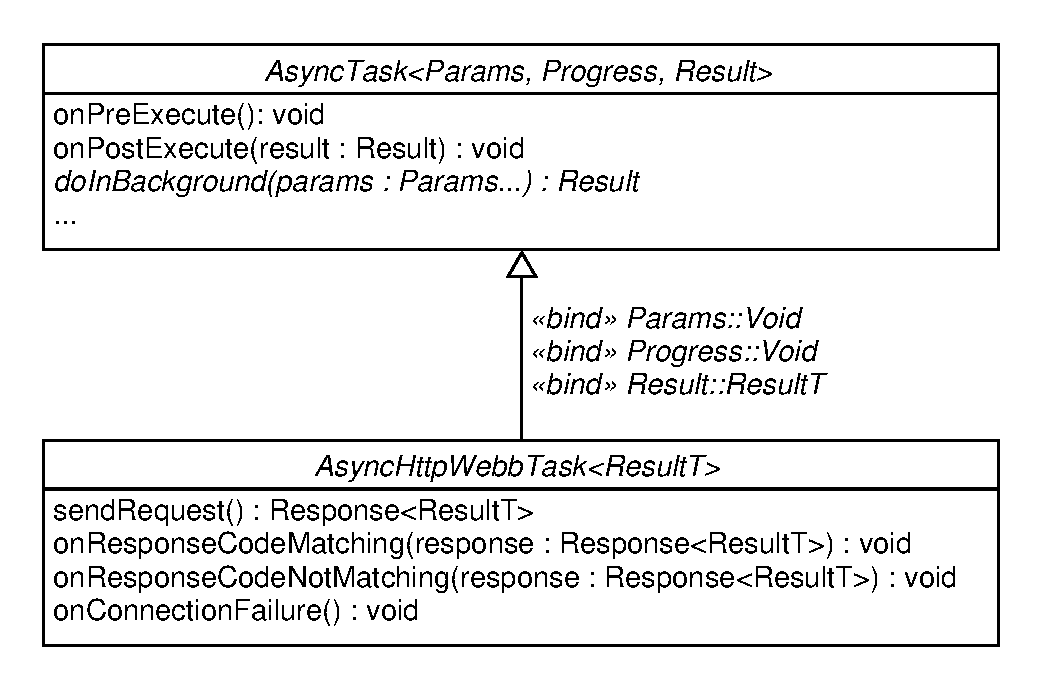
\includegraphics[width=0.5\textwidth]{graphic/architecture/async_http_webb_task.pdf}
    \caption{An UML diagram describing the class extending the AsyncTask.}
    \label{fig:async_http_webb_task}
\end{figure}
\FloatBarrier

We found that we needed to ensure that the response code matches what we expected in the different situations, such as 200 (status OK), and would otherwise need to make some error handling. We also figured that we often would need to specify what to happen if there were no available connection to the server, such that there were no response code returned. Therefore we overrode the \mono{onPostExecute} method as seen in \lstref{lst:on_post_execute}. 

\lstinputlisting[
   style = Java,
   caption = {The \mono{onPostExecute} method, which is called after the asynchronous task has completed.},
   label = {lst:on_post_execute},
   float=!htbp,
]{content/architecture/code_snippets/onPostExecute.java}
\FloatBarrier

Here we firstly check if the response parameter is null, in which case something went wrong in establishing the connection to the server, and the abstract method \mono{onConnectionFailure} will be called. Otherwise we check if the response code matches what we expect, and if it is we call the abstract method \mono{onResponseCodeMatching} and if it does not we call \mono{onResponseCodeNotMatching}. These methods can then be overridden in an anonymous class or a normal class. The response code from the snippet is set through the constructor of the method, along with the the URL the request should be sent to and the request method, which is either ``GET'', ``POST'', ``PUT'', or ``DELETE''. 

\todo[inline]{Skal vi beskrive disse HTTP request typer?}.

The response that the \mono{onPostExecute} in \lstref{lst:on_post_execute} receives as an argument is the result of the doInBackground process, which can be seen in \lstref{lst:do_in_background}. 

\lstinputlisting[
   style = Java,
   caption = {The actual task being executed on a background thread.},
   label = {lst:do_in_background},
   float=!htbp,
]{content/architecture/code_snippets/doInBackground.java}
\FloatBarrier

In this method we firstly create a custom \mono{TrustManager} and \mono{HostnameVerifier}, which is connected to the Transport Layer Security that we utilize and will be described in \secref{sec:transport_layer_security}. This is followed by setting some of the properties that we want to apply to every request, such as adding the ``X-requested-with''-header describing that the request is an Ajax request and not a normal web page request. This is followed by a check of which method is requested in the constructor and use the Webb library to create a request of that type, and use it as a parameter for the abstract method called sendRequest. As with the other abstract methods the \mono{sendRequest} method can be overridden to specify different aspects of the request, such as what the parameters for the request should be as well as how many reties there should be.

\subsection{Request Handling}
\label{sub:request_handling}
In the architecture a request from device is going through two different handlers when the server receives it. Firstly it is registered by the NGINX Web Server, which listens on port 8000. Then it will be determined by the webserver which virtual server should handle the request. A virtual server is defined inside the nginx configuration files, where we for one physical server can specify that it should listen on multiple ports and even have more than one web site listening on the same port, where the requested server name, e.g. www.example.com, determines which of the virtual servers should handle the request. In our case we have two different virtual servers. One for development and one for production. These two virtual servers (server blocks) have been defined in their own configuration file, which then is included by the main configuration file of nginx. An example of the configuration file for our production site can be seen in \lstref{lst:server_conf}. 

\lstinputlisting[
   caption = {NGINX server configuration.},
   label = {lst:server_conf},
   float=!htbp,
]{content/architecture/code_snippets/server.conf}
\FloatBarrier

In line \linesref{lst:server_conf_listen_begin}{lst:server_conf_listen_end} the port that the server should listen on is specified. In our case it would have been ideal to utilize port 80, but the port was already occupied by another server using external IP that was granted to us by the university, instead we were assigned port 8000, which is the one that we utilize as seen in the snippet. This is followed by a directive specifying the root folder of the web site in \lineref{lst:server_conf_root}, and then the index directive specifying that it should prioritize to serve a page called index.php over its HTML counterpart. The server\_name directive was covered by the earlier example, and in this case we are looking at the production server configuration and therefore the names are ``prod.local.element67.dk'' and ``prod.global.element67.dk''. The two location directives as seen in \lineref{lst:server_conf_location} and \lineref{lst:server_conf_location2_begin} specify which page the server should try to serve (relative to the root path) and how it should be done. The syntax for these declarations is the location keyword followed by an optional ``modifier'' and lastly the ``location match'' that the requested URL should match. There are different possibilities for modifiers. In the case of the first location in \lstref{lst:server_conf} we utilize no modifier, meaning that it should be a prefix match. In the case of a prefix match it will try to match the beginning of the given URI (the URL without the hostname in this case) to the location match, and due to the fact that it is a prefix match and the location match is ``/'', all request will be captured by this one, because every URL is prefixed by the root. The second locations modifier is tilde (\~ ), meaning that the location match will match with a case-sensitive regular expression. The regular expression in the second location match every request with a \mono{.php} suffix in the URI and thereby the directive will capture all requests that is made to a PHP file.
\\\\
When a request is handled by NGINX it will try to find the most specific match, meaning that it will always fall back to the location with the location match of ``/''. Inside this location it will then be checked if it is possible to find a file matching the exact name specified, and if that is not possible we will try to match on folder, and see if that folder contains an index file as specified in the index directive in \lineref{lst:server_conf_index}. If that is not possible the request will internally be redirected to the \mono{index.php} file in the document root, along with any potential query string. This redirection will then be captured by the second location directive in \lineref{lst:server_conf_location2_begin}. This location will as previously mentioned capture all request made to the any PHP files in the system. If any matches the it will choose to use that one, otherwise it will find the index.php file in the root directory and send it this file to the PHP FastCGI Process manager, which runs on a unix socket. An illustration of how a specific request is handled by NGINX is shown in \figref{fig:nginx_workflow}.

\begin{figure}[!htbp]
    \centering
    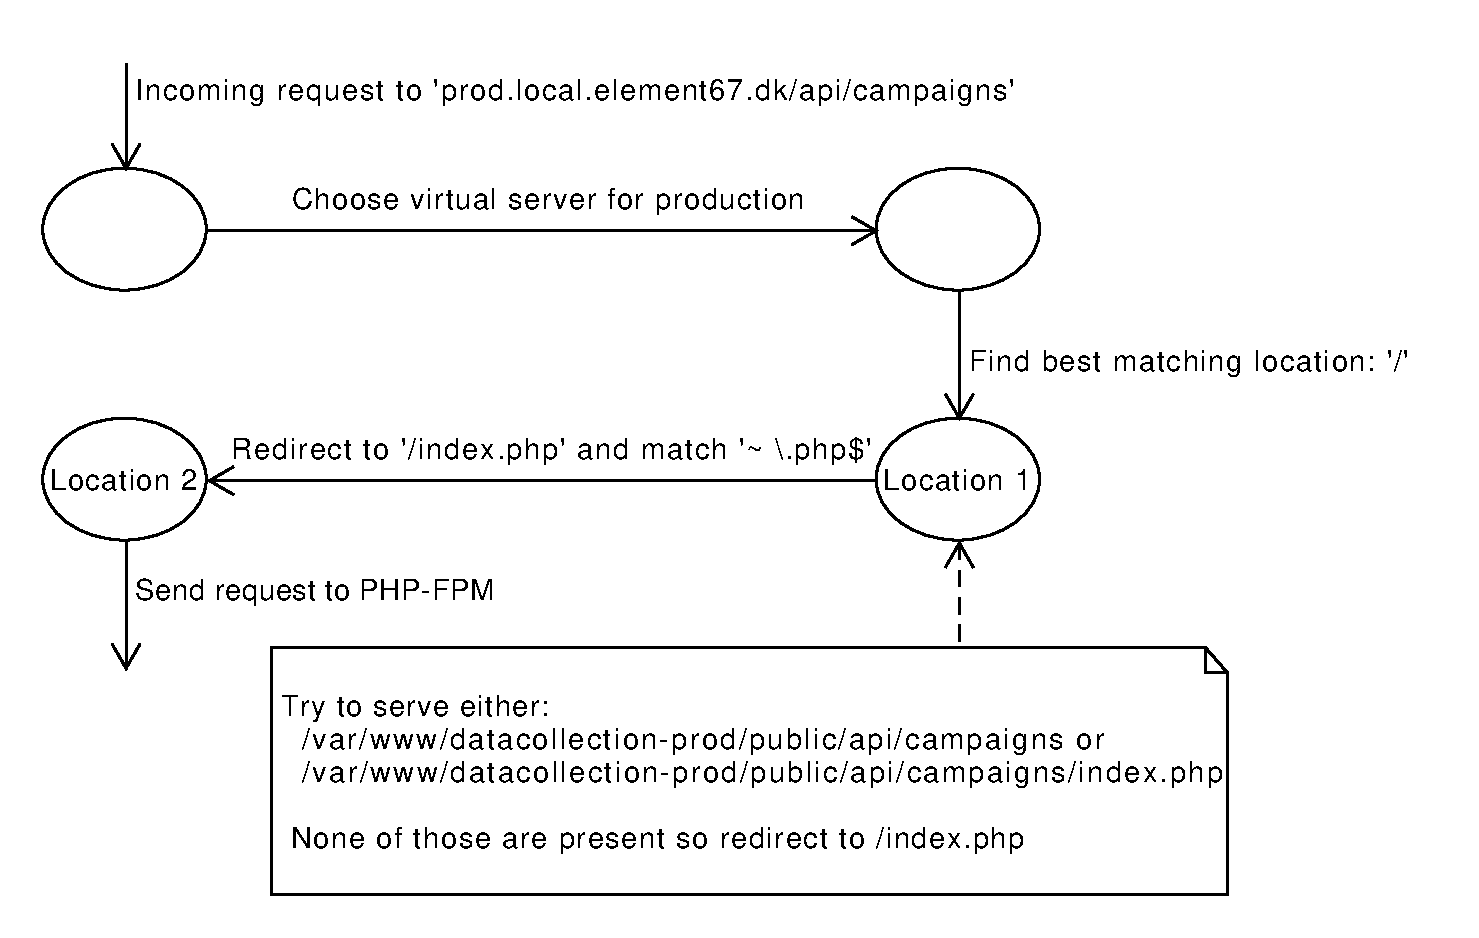
\includegraphics[width=0.7\textwidth]{graphic/architecture/nginx_workflow.pdf}
    \caption{An example of how a request could be handled by nginx with our configuration.}
    \label{fig:nginx_workflow}
\end{figure}
\FloatBarrier

Firstly a request is sent to ``prod.local.element67.dk/api/campaigns'', and NGINX will then decide which virtual server should handle the request. In this case it will be the one specified in \lstref{lst:server_conf}, and it will find the best matching location. The request does not have the PHP suffix, so it is captured by the general location. Neither the file or the index file in the directory does in this hypothetical case exist. Therefore the request is internally redirected to ``/index.php'', and is forwarded to the PHP FPM unix socket, where the PHP interpreter and Laravel will take over. 
\\\\
The entry point for the Laravel framework is through the ``index.php'' file that NGINX just redirected to. Here it will will create its own Request object from the request it received from NGINX. This request object is then send to a handler which initiates the flow shown in \figref{fig:laravel_flow}. This flow shows that Laravel utilizes a MVC architecture.

\begin{figure}[!htbp]
    \centering
    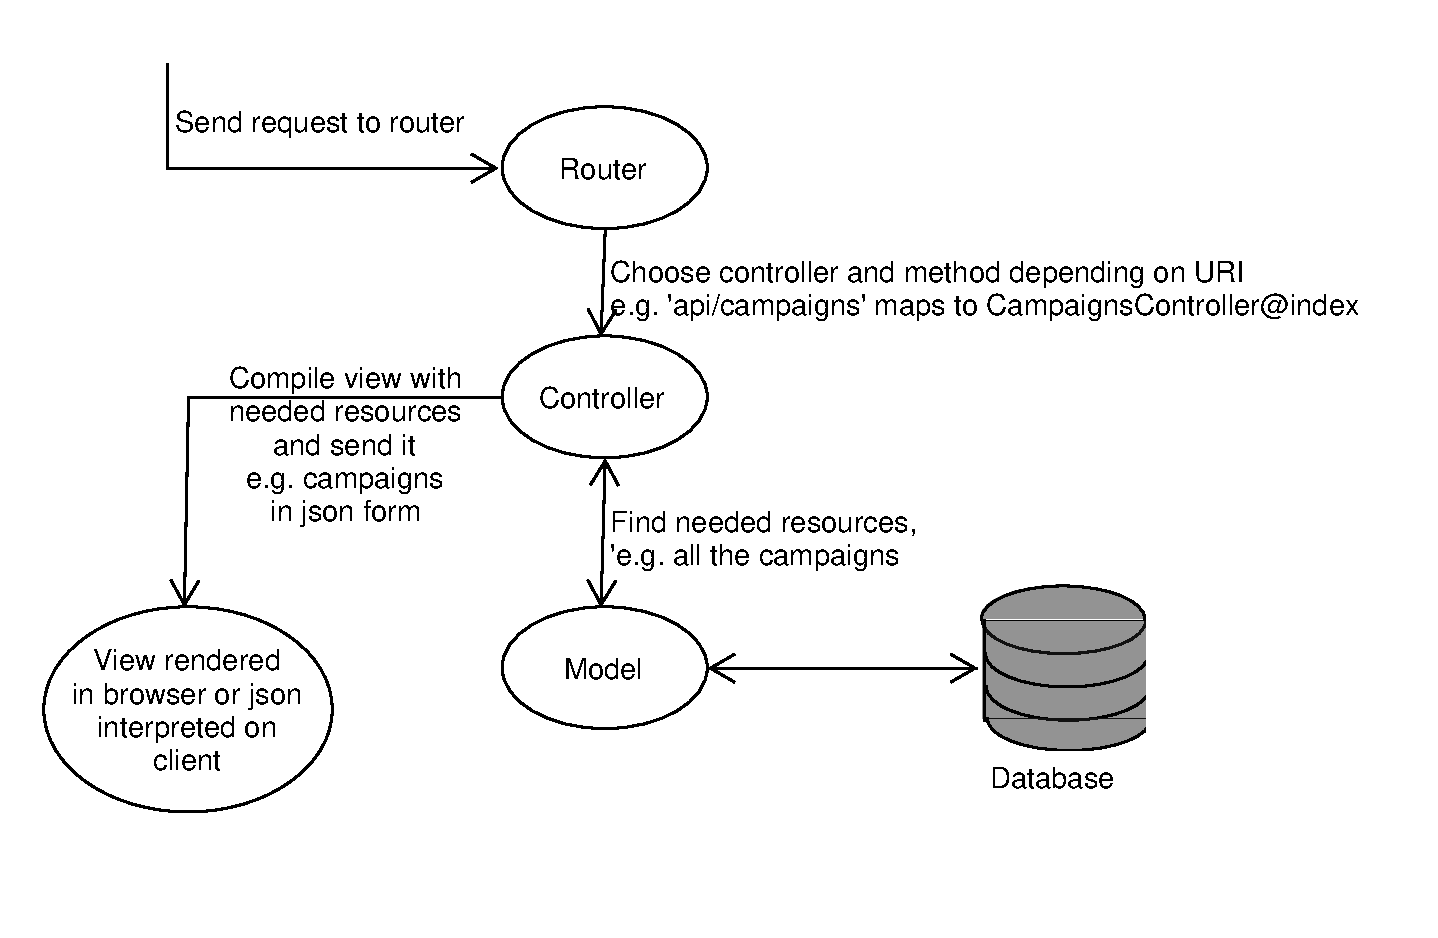
\includegraphics[width=0.7\textwidth]{graphic/architecture/laravel_flow.pdf}
    \caption{An illustration of how a request is traverses through Laravel.}
    \label{fig:laravel_flow}
\end{figure}

Firstly the request is send to the router, which looks at the initial request URI (the URI before NGINX redirected is still available in the HTTP header). Then the router determines which controller-method should be called, retrieves any parameters captured by wildcards in the URI, and invoke the controller-method with these. It is then the controllers job to fetch the needed models to create the requested view, which in the case of an api route will be a JSON response of the given models. The JSON response will then be interpreted by the Android client and the requested information will be shown to the user. 
% https://www.digitalocean.com/community/tutorials/how-to-install-laravel-with-an-nginx-web-server-on-ubuntu-14-04
% https://www.digitalocean.com/community/tutorials/understanding-nginx-server-and-location-block-selection-algorithms
% http://nginx.org/en/docs/http/request_processing.html
